\begin{boxC}
    در تصاویر زیر می‌توانید دقت‌ این مدل به ازای 
    \lr{label}
    های مختلف را مشاهده‌بفرمایید.

    \begin{itemize}
        \item 
        خیر. تعداد تگ‌های هر دسته متعادل نمی‌باشد.
        تعداد و میزان هر تگ را می‌توان از نمودار پایین مشاهده نمود.
        بیشترین تگ مربوط به تگ مثبت و کمترین تگ مربوط به تگ خنثی می‌باشد.


        \item 
        معماری :
        در واقع مدل ما در ۳ ایپاک آموزش دیده است.
        بر اساس دو معیار زیر که اولی به میزان جریمه ، و دومی به میزان دقت اشاره می‌کند ، به آموزش مدل خود بر حسب داده آموزشی می‌پردازیم.
        
        \lr{loss = tf.keras.losses.SparseCategoricalCrossentropy(fromlogits=True)}
        \newline
        \lr{metric = tf.keras.metrics.SparseCategoricalAccuracy('accuracy')}
        % \newline

        سپس با استفاده از کد زیر بهترین وزن‌دهی‌ها را ذخیره خواهیم کرد.

        \lr{bertmodel.saveweights(modelsavepath)}

        \item 
        با توجه به نمودارهای زیر مشخص است که مدل آموزش دیده دچار بیش برازش نشده است ، چرا که هیچ گونه اثری از انطباق بر روی نمودار آموزش و اعتبارسنجی مشاهده نمی‌شود.

        \item 
        مراحل ذکر شده در داکیومنت تمرین چهارم به صورت دقیق در کد ، پیاده‌سازی گردیده‌است.
        همچنین توضیحات مختصری در قالب کامنت در سلول‌های 
        \lr{Text}
        قرار داده‌شده‌است.
        
    \end{itemize}
\end{boxC}

\begin{boxK}
    نکته جالبی که می‌توان به آن اشاره کرد این است که در قسمت تابع ضرر
    (\lr{Loss Function})
    در صورتی که یکی از تگ های داده را به یک عدد منفی مثل -۱ نظیر کنیم ، به شدت میزان دقت مدل کاهش می‌یابد.
    (نتیجه‌ای که شخصا به آن رسیدم این بود که این تابع محاسبه ضرر به ازای منفی بودن تگ‌ها به شدت دقت پایینی را محاسبه خواهد کرد ، به طوری که دقت مدل من در حدود ۱۵ درصد بوده است.)
\end{boxK}

\begin{figure}[h]
    \centering
    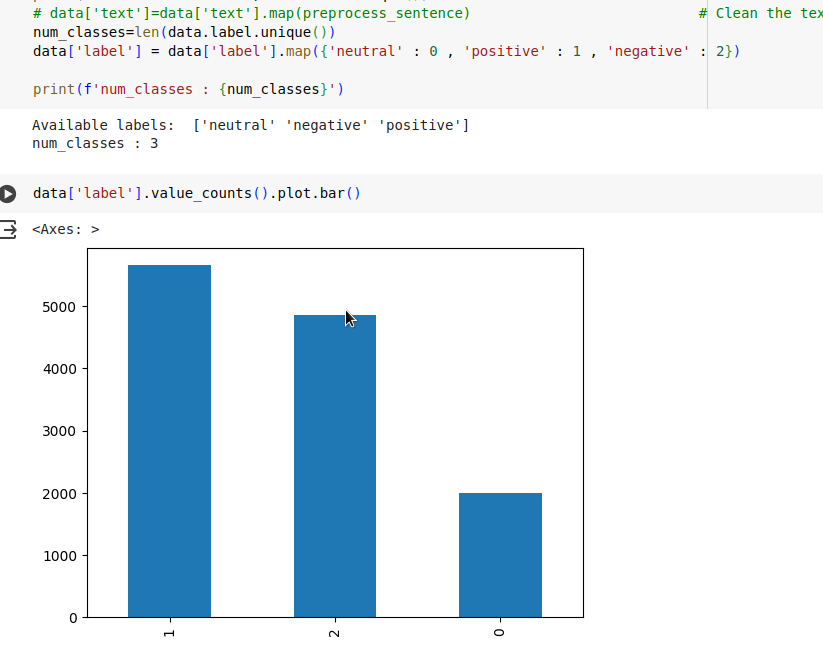
\includegraphics
    [width = 0.8 \textwidth]
    {IR4/images/labels.png}
    \caption{\lr{All labels in dataset}}
    \label{fig:enter-label}
\end{figure}

\begin{figure}[h]
        \centering
        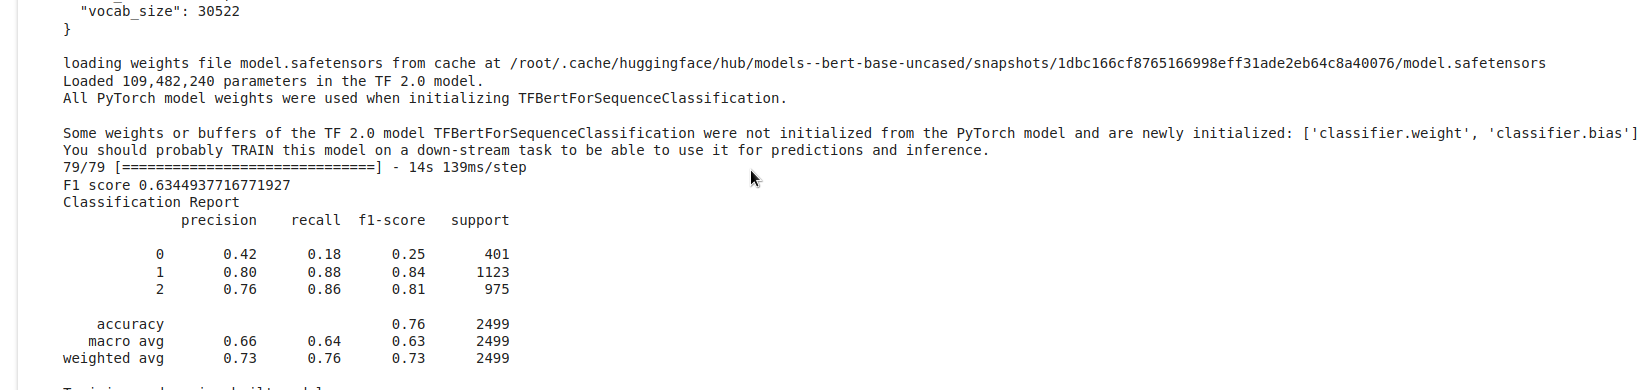
\includegraphics
        [width = 0.9\textwidth]
        {IR4/images/all-scores.png}
        \caption{ همه مقیاس‌های مدنظر}
        \label{fig:enter-label}
\end{figure}

\begin{figure}[h]
        \centering
        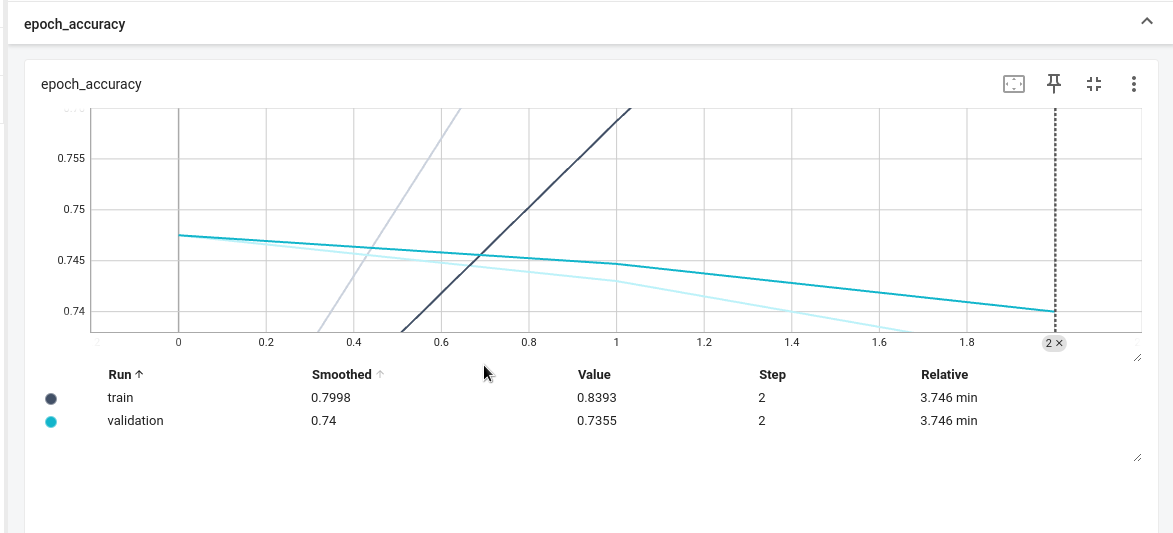
\includegraphics
        [width = 0.8\textwidth]
        {IR4/images/tensorflow_accuracy.png}
        \caption{\lr{tensorflow accuracy}}
        \label{fig:enter-label}
\end{figure}

\begin{figure}[h]
        \centering
        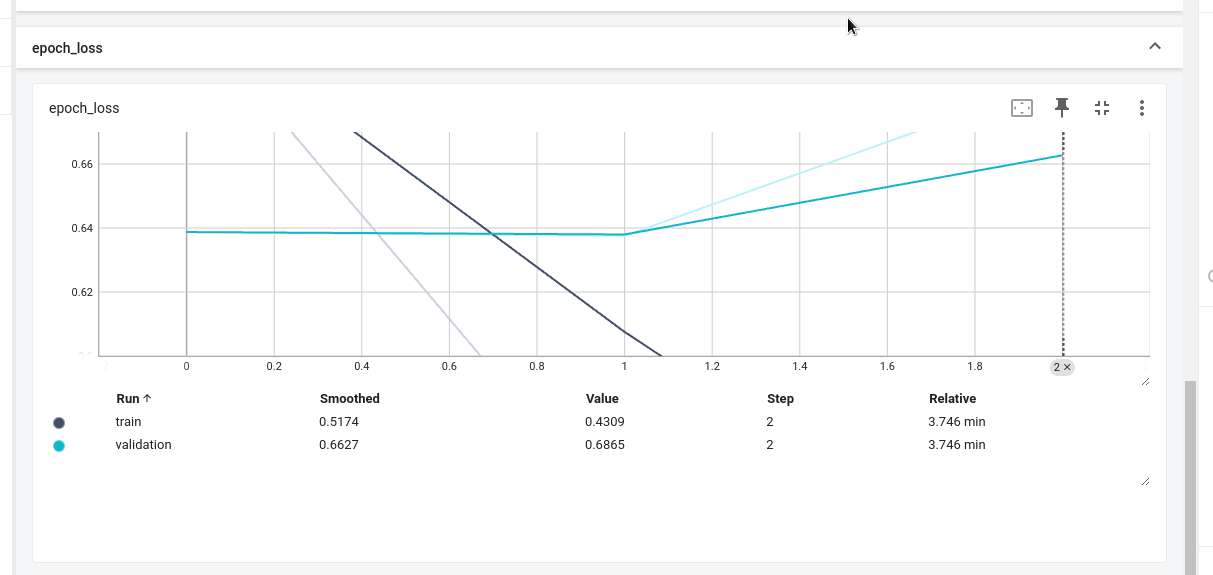
\includegraphics
        [width = 0.8\textwidth]
        {IR4/images/tensorflow-loss.png}
        \caption{\lr{tensorflow loss}}
        \label{fig:enter-label}
\end{figure}

\clearpage